\begin{apartats}

\apartat[1,25]{0,75}
Calcula les integrals indefinides $\displaystyle\int(3x^2-4x+1)\,dx$ i $\displaystyle\int(x-2)^3\,dx$.

\begin{solucio}
$\displaystyle\int(3x^2-4x+1)\,dx=x^3-2x^2+x+k$ i $\displaystyle\int(x-2)^3\,dx=\frac{(x-2)^4}{4}+k$.
\end{solucio}

\begin{tria}{integral-definida}
\itemtria{barrow}{1}{1,25}
Calcula $\displaystyle\int_0^2(3x^2-4x+1)\,dx$ i $\displaystyle\int_1^3(x-2)^3\,dx$. Per què la segona val 0?

\begin{solucio}
Per la regla de Barrow:
$\displaystyle\int_0^2(3x^2-4x+1)\,dx=\bigl[x^3-2x^2+x\bigr]_0^2=(8-8+2)-0=2$ i
$\displaystyle\int_1^3(x-2)^3\,dx=\left[\frac{(x-2)^4}{4}\right]_1^3=\frac14-\frac14=0$.\\
La funció $(x-2)^3$ és negativa a $[1,2]$ i positiva a $[2,3]$, i les dues regions són iguals
(simètriques respecte del punt $(2,0)$): les seves contribucions es compensen.
\end{solucio}

\itemtria{grafica}{1}{1,25}
La gràfica de la funció $f$ és la del dibuix. Calcula, sense buscar-ne cap primitiva,
$\displaystyle\int_{-2}^4 f(x)\,dx$ i $\displaystyle\int_0^3 f(x)\,dx$.
\begin{center}
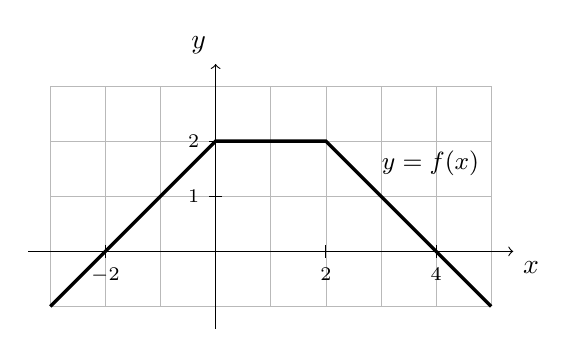
\begin{tikzpicture}[x=0.7cm,y=0.7cm]
  \draw[gray!55,very thin,step=1] (-3,-1) grid (5,3);
  \draw[->] (-3.4,0) -- (5.4,0) node[below right] {$x$};
  \draw[->] (0,-1.4) -- (0,3.4) node[above left] {$y$};
  \foreach \i in {-2,2,4} \draw (\i,0.12) -- (\i,-0.12) node[below,font=\scriptsize] {$\i$};
  \foreach \j in {1,2} \draw (0.12,\j) -- (-0.12,\j) node[left,font=\scriptsize] {$\j$};
  \draw[\colorgrafica,very thick] (-3,-1) -- (0,2) -- (2,2) -- (5,-1);
  \node[\colorgrafica,font=\small] at (3.9,1.6) {$y=f(x)$};
\end{tikzpicture}
\end{center}

\begin{solucio}
Entre $-2$ i $4$, $f\ge0$, i la integral és l'àrea sota la gràfica: un triangle de base 2 i altura 2, un
rectangle $2\times2$ i un altre triangle igual. $\displaystyle\int_{-2}^4 f(x)\,dx=2+4+2=8$.\\
Entre 0 i 3: el rectangle, 4, més el trapezi de bases 2 i 1 i altura 1, $\frac{2+1}2=1{,}5$. En total,
$5{,}5$.
\end{solucio}
\end{tria}

\begin{nomesllarg}
\apartat{0,75}
Sabent que $\displaystyle\int_0^3 g(x)\,dx=5$ i $\displaystyle\int_0^3 h(x)\,dx=-2$, calcula
$\displaystyle\int_0^3\bigl(2g(x)-3h(x)\bigr)\,dx$ i $\displaystyle\int_3^0 g(x)\,dx$.

\begin{solucio}
Per la linealitat de la integral, $2\cdot5-3\cdot(-2)=16$. Canviar l'ordre dels límits canvia el signe:
$\displaystyle\int_3^0 g(x)\,dx=-5$.
\end{solucio}
\end{nomesllarg}

\end{apartats}
